\documentclass[a4paper]{article}
\usepackage[utf8]{inputenc} % Skal passe til editorens indstillinger
\usepackage[english]{babel} % danske overskrifter


\newcommand{\name}{Carsten Nielsen}
%\newcommand{\stnumber}{s123369, s123161, s123821}
\newcommand{\course}{INI 404 Neuromorphic Engineering~I}
\newcommand{\university}{University of Zürich}
\newcommand{\studyline}{Institute of Neuroinformatics}
\newcommand{\assignment}{Lab 8 Post-Lab}
\renewcommand{\date}{\today} %If another date, than that of today is desiered


% Palatino for rm and math | Helvetica for ss | Courier for tt
\usepackage{mathpazo} % math & rm
\linespread{1.05}        % Palatino needs more leading (space between lines)
\usepackage{palatino} % tt
\normalfont
\usepackage[T1]{fontenc}
\usepackage[english]{babel}

\usepackage{graphicx}%allerese hentet % indsættelse af billeder
\usepackage{epstopdf} %Tilfj "--enable-write18" i argumentet for LaTex build. Dette vil konvertere .eps figurer til pdf-format
\graphicspath{{./picture/}} % stivej til bibliotek med figurer
\usepackage{subcaption} %Til gruppering af figurer
\usepackage{amsmath} %matpakke
\usepackage{amsfonts} %
\usepackage{amssymb} %
\usepackage{steinmetz} % flere matematik symboler
\usepackage{polynom} %for displaying polynom division
\usepackage{mathtools} % matematik - understøtter muligheden for at bruge \eqref{}
\usepackage{float}
\usepackage{placeins}
\usepackage{hhline}

%
\usepackage[usenames,dvipsnames]{xcolor}
\usepackage[compact,explicit]{titlesec}% http://ctan.org/pkg/titlesec
%
\usepackage[europeanresistors]{circuitikz}
\usepackage{pgfplots}
\usepgfplotslibrary{patchplots}
\pgfplotsset{compat=1.11}

%---------%
%Easy edit%
%---------%

%Section formating. arg1 is supplied when making section
\newcommand\presectionnumber[1]{~~}
\newcommand\postsectionnumber[1]{}
\newcommand\midlesection[1]{#1}
\newcommand\sectionnum[1]{\arabic{#1}}
\newcommand\subsectionnum[1]{\arabic{#1}}
\newcommand\subsubsectionnum[1]{\alph{#1}}



%------------%
%setion setup%
%------------%
\renewcommand\thesection{Opgave~\sectionnum{section}} %pas p�, kun i matematik
\renewcommand\thesubsection{\thesection,~\subsectionnum{subsection}}
\definecolor{MagRed}{RGB}{190,40,15}
\definecolor{MathGreen}{RGB}{82,164,0}

\titleformat{\section}{\normalfont\sffamily\large\bfseries\color{MathGreen}}{}{0pt}{|\kern-0.15ex|\kern-0.15ex|\kern-0.15ex|\presectionnumber{#1}\sectionnum{section}\postsectionnumber{#1}\qquad\quad\midlesection{#1}\label{sec:\sectionnum{section}}}
\titleformat{\subsection}[runin]{\large\bfseries}{}{10pt}{\sectionnum{section}.\subsectionnum{subsection})~#1\label{sec:\sectionnum{section}.\subsectionnum{subsection}}}
\titleformat{\subsubsection}[runin]{\itshape}{}{0pt}{\subsectionnum{subsection},\subsubsectionnum{subsection}~#1\label{sec:\sectionnum{section}.\subsectionnum{subsection}.\subsubsectionnum{subsubsection}}}
%\titleformat{\subsubsection}{\bfseries}{}{0pt}{\alph{subsection}.\arabic{subsubsection})\qquad\quad#1\label{\arabic{section}\alph{subsection}\arabic{subsubsection}}}

%----------%
%page setup%
%----------%
\textwidth = 400pt
\marginparwidth = 86pt
\hoffset = -25pt
\voffset= -30pt
\textheight = 670pt

%--------%
%hyperref%
%--------%
\newcommand{\HRule}{\rule{\linewidth}{0.5mm}}
\usepackage{fancyhdr}
\usepackage[plainpages=false,pdfpagelabels,pageanchor=false]{hyperref} % aktive links
\hypersetup{%
  pdfauthor={\name},
  pdftitle={\assignment},
  pdfsubject={\course} }
%\usepackage{memhfixc}% rettelser til hyperref

%-------------%
%Headder setup%
%-------------%
\fancyhf{} % tom header/footer
\fancyhfoffset{20pt}
\fancyhfoffset{20pt}
\fancyhead[OL]{\name \\ INI 404}
\fancyhead[OC]{Date \\ \date}
\fancyhead[OR]{\university\\ \studyline}
\fancyfoot[FL]{}
\fancyfoot[FC]{\thepage}
\fancyfoot[FR]{}
\renewcommand{\headrulewidth}{0.4pt}
\renewcommand{\footrulewidth}{0.4pt}
\headsep = 35pt
\pagestyle{fancy}
 % style setup

%Listings%
\usepackage{listingsutf8}
\usepackage[framed,numbered]{matlab-prettifier}


%setup listings
\lstset{language=Matlab,
  extendedchars=true,
  language=Octave,                % the language of the code
  basicstyle=\ttfamily\footnotesize,           % the size of the fonts that are
  % used for the code
  numbers=left,                   % where to put the line-numbers
  numberstyle=\tiny\color{gray},  % the style that is used for the line-numbers
  stepnumber=2,                   % the step between two line-numbers. If it's 1, each line 
                                  % will be numbered
  numbersep=5pt,                  % how far the line-numbers are from the code
  backgroundcolor=\color{white},      % choose the background color. You must add \usepackage{color}
  showspaces=false,               % show spaces adding particular underscores
  showstringspaces=false,         % underline spaces within strings
  showtabs=false,                 % show tabs within strings adding particular underscores
  frame=single,                   % adds a frame around the code
  rulecolor=\color{black},        % if not set, the frame-color may be changed on line-breaks within not-black text (e.g. comments (green here))
  tabsize=4,                      % sets default tabsize to 2 spaces
  captionpos=b,                   % sets the caption-position to bottom
  breaklines=true,                % sets automatic line breaking
  breakatwhitespace=false,        % sets if automatic breaks should only happen at whitespace
  title=\lstname,                   % show the filename of files included with \lstinputlisting;
                                  % also try caption instead of title
  %keywordstyle=\color{blue},          % keyword style
  %commentstyle=\color{dkgreen},       % comment style
  %stringstyle=\color{mauve},         % string literal style
  escapeinside={\%*}{*)},            % if you want to add LaTeX within your code
  morekeywords={*,...},              % if you want to add more keywords to the set
  deletekeywords={...}              % if you want to delete keywords from the given language
}
\lstset{literate=
  {á}{{\'a}}1 {é}{{\'e}}1 {í}{{\'i}}1 {ó}{{\'o}}1 {ú}{{\'u}}1
  {Á}{{\'A}}1 {É}{{\'E}}1 {Í}{{\'I}}1 {Ó}{{\'O}}1 {Ú}{{\'U}}1
  {à}{{\`a}}1 {è}{{\`e}}1 {ì}{{\`i}}1 {ò}{{\`o}}1 {ù}{{\`u}}1
  {À}{{\`A}}1 {È}{{\'E}}1 {Ì}{{\`I}}1 {Ò}{{\`O}}1 {Ù}{{\`U}}1
  {ä}{{\"a}}1 {ë}{{\"e}}1 {ï}{{\"i}}1 {ö}{{\"o}}1 {ü}{{\"u}}1
  {Ä}{{\"A}}1 {Ë}{{\"E}}1 {Ï}{{\"I}}1 {Ö}{{\"O}}1 {Ü}{{\"U}}1
  {â}{{\^a}}1 {ê}{{\^e}}1 {î}{{\^i}}1 {ô}{{\^o}}1 {û}{{\^u}}1
  {Â}{{\^A}}1 {Ê}{{\^E}}1 {Î}{{\^I}}1 {Ô}{{\^O}}1 {Û}{{\^U}}1
  {œ}{{\oe}}1 {Œ}{{\OE}}1 {æ}{{\ae}}1 {Æ}{{\AE}}1 {ß}{{\ss}}1
  {ç}{{\c c}}1 {Ç}{{\c C}}1 {ø}{{\o}}1 {å}{{\r a}}1 {Å}{{\r A}}1
  {€}{{\EUR}}1 {£}{{\pounds}}1
}

 \lstloadlanguages{% Check Dokumentation for further languages ...
         %[Visual]Basic
         %Pascal
         %C
         %C++
         %XML
         %HTML
         %Java
         %VHDL
         Matlab
 }
 %Listings slut%









%Matematik hurtige ting
%fed
\renewcommand\vec[1]{\mathbf{#1}}
\newcommand\matr[3]{{}_{#2}\mathbf{#1}{}_{#3}}
\newcommand\facit[1]{\underline{\underline{#1}}}
%\renewcommand\d[3]{\frac{\mbox{d}^{#3}#1(#2)}{\mbox{d}#2^{#3}}}
%underline
%\renewcommand\vec[1]{\underline{#1}}
%\newcommand\matr[3]{{}_{#2}\underline{\underline{#1}}{}_{#3}}

\renewcommand\matrix[4]{ %{alignment}{to space}{from space}{matrix}
{\vphantom{\left[\begin{array}{#1}#4\end{array}\right]}}_{#2}\kern-0.5ex
\left[\begin{array}{#1}
#4
\end{array}\right]_{#3}
}
\newcommand\e[0]{\mbox{e}}
\newcommand\E[1]{\cdot 10^{#1}}
\newcommand\im[0]{i}

\newcommand\Jaco{\mbox{Jacobi}}
\newcommand\del[2]{\frac{\partial {#1}}{\partial {#2}}}
\newcommand\abs[1]{\left| {#1} \right|}
\newcommand\stdfig[4]{ %width,img,cap,lab
\begin{figure}[H]
\centering
\includegraphics[width={#1}\textwidth]{#2}
\caption{#3}
\label{#4}
\end{figure}
}
\newcommand\stdfignoscale[3]{ %img,cap,lab
\begin{figure}[H]
\centering
\includegraphics{#1}
\caption{#2}
\label{#3}
\end{figure}
}
\newcommand\diff{\dot}
\newcommand\ddiff{\ddot}
\newcommand\dddiff{\dddot}
\newcommand\ddddiff{\ddddot}






% How to make ref to books or urls in bib
%\citetitle[fx: page 1]{name of ref in bib}


\tikzset{rrail/.style={rground,yscale=-1}}
\newcommand{\reffig}[1]{Fig.~\ref{#1}}

\begin{document}
\begin{titlepage}
\centering \parindent=0pt

\vspace*{\stretch{1}} \HRule\\[1cm]\Huge
\course\\[0.7cm]
\large \assignment\\[1cm]
\HRule\\[4cm]  
%\includegraphics[width=6cm]{picture}\\ Use this if you want a picture on the frontpage
\name\\
%\stnumber
TAs: Ning Quiao, Chenghan Li

\vspace*{\stretch{2}} \normalsize %

\begin{center}
	\date 
\end{center}
\vspace*{\stretch{2}} \normalsize
\begin{flushright}
%\includegraphics[width=6cm]{./dtu.eps}\\
\end{flushright}
\end{titlepage}

\newpage
\section{Experiment 1}
\begin{figure}
    \begin{subfigure}{0.5\textwidth}
        \center
        \begin{circuitikz}[american voltages] \draw
            (0,0) node[nmos] (mos) {}
            (mos.base) node[anchor=west] {} -- (1,0) to[short] (1,-1)
            (1,-1) node[ground] {} (1,-1)
            (-1.5,-1) to[V] (-1.5,-0) -- (mos.gate)
            (mos.gate) node[anchor=east] {} 
            (-1.5,-1) node[ground] {} (-1.5,-1)
            (mos.drain) node[anchor=south] {} -- (0, 1)
            (0,1) node[rrail] {}
            node[right] {$V_{dd}$}
            (mos.source) node[anchor=north] {} to[ammeter=K236, name=M] (0,-2)
            (0,-2) node[ground] {} to (0,-2)
            (-2,-0.5) node[anchor=east] {K230}
            (-0.3, -1.5) node[anchor=east] {K236}
        ;\end{circuitikz}
        \caption{}
    \end{subfigure}
    \begin{subfigure}{0.5\textwidth}
        \center
        \begin{circuitikz}[american voltages] \draw
            (0,0) node[pmos] (mos) {}
            (mos.base) node[anchor=west] {} -- (1,0) to[short] (1,1)
            (1,1) node[rrail] {} (1,1)
            (mos.gate) -- (-1.5,0) to[V] (-1.5,1) node[rrail] {}
            (mos.gate) node[anchor=east] {} 
            (mos.source) node[anchor=south] {} -- (0, 1)
            (0,1) node[rrail] {}
            node[right] {$V_{dd}$}
            (mos.drain) node[anchor=north] {} to[ammeter=K236, name=M] (0,-2)
            (0,-2) node[ground] {} to (0,-2)
            (-2,0.5) node[anchor=east] {K230}
            (-0.3, -1.5) node[anchor=east] {K236}
        ;\end{circuitikz}
        \caption{}
    \end{subfigure}
    \caption{Experimental setup for experiment 1. We measured \(I_{ds}\) at the source terminal of the native nMOS transistor (a)
    and drain terminal of the well type pMOS transistor (b).}
    \label{fig:setup1}
\end{figure}
\begin{figure}
    \center
    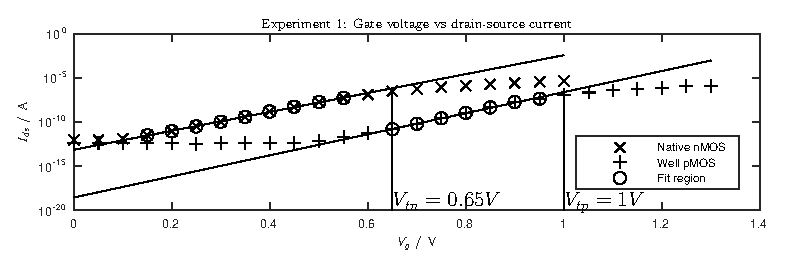
\includegraphics{ex1.eps}
    \caption{\(I_{ds}\) as a function of the gate voltage \(V_g\) for the native nMOS and well type pMOS transistors. Lines are linear fits
    to the points marked with circles. The threshold voltages \(V_{tn}=0.65\) V and \(V_{tp} = 1\) V are also marked.}
    \label{fig:ex1}
\end{figure}
We measured the \(I_{ds}\) currents of both the native and well transistors using the setups shown in \reffig{fig:setup1}. Our measurements 
can be seen in \reffig{fig:ex1}. The fitted lines have the following equations:
\begin{align*}
    I_{dsn} & = e^{-30.25}e^{24.68V_g} \\
    I_{dsp} & = e^{-42.71}e^{27.5V_g} 
\end{align*}
For the native nMOS and well type pMOS respectively.

Since the current through the transistor in the subtreshold region can be described by the equation
\begin{equation*}
    I_{ds} = I_0e^{\frac{\kappa V_g}{U_t}}\left(e^{\frac{-V_s}{U_t}}-e^{\frac{-V_d}{U_t}}\right)
\end{equation*}
We can find \(I_0\) and \(\kappa\) from the fitted equations above, assuming \(U_t=26\) mV.
\begin{align*}
    I_{n0} = e^{-30.25} & = 72.9\text{ fA} \quad \kappa_n = 0.64 \\
    I_{p0} = e^{-42.71} & = 0.28\text{ aA} \quad \kappa_p = 0.72
\end{align*}
The extrapolated \(\kappa\) values are too low, which is likely due to the \(U_t=26\) mV assumption not being valid as it
depends on the temperature of the junction which we do not know. The extrapolated values for the quiescent currents are also 
much lower than what we measure. We measure 
\begin{equation*}
    I_{n0} = 84 \text{ pA} \quad I_{p0} = 39 \text{ pA}
\end{equation*}
This number includes the leakage current and noise, and is larger for the nMOS transistor because electrons have higher mobility than holes.
Additionally, the SMU is not capable of measuring currents as low as predicted by the theoretical fits.

We measure threshold currents
\begin{equation*}
    I_{nt} = 29.3 \mu \text{A} \quad I_{pt} = 10.9 \mu \text{A}
\end{equation*}
With the ratio \(\frac{I_{nt}}{I_{pt}}=2.69\) which is the relative mobility of electrons and holes. Ideally this should be 2.5.
\section{Experiment 2}
We use the measurement setup shown in \reffig{fig:setup2} to measure \(V_s\) as a function of \(V_g\) when a constant current of
1 nA is forced through the transistor. The results for both transistors can be seen in \reffig{fig:ex2vsvg}. The lines
are linear fits and the slope of the lines are the \(\kappa\) values for the nMOS and pMOS transistors.
This result can be derived by considering the current in saturation mode \(e^{\frac{-V_{ds}}{U_t}} \sim 0\)
\begin{equation*}
    I_{ds} = I_0e^{\frac{\kappa V_g - V_s}{U_t}}
\end{equation*}
Since we are forcing a constant current \(I_f\) through the transistor we have
\begin{align*}
    I_f & = I_0e^{\frac{\kappa V_g - V_s}{U_t}} \\
        &\Updownarrow \\
    V_s &= \kappa V_g - \frac{\ln\left(I_f\right)}{\ln\left(I_0\right)}U_T \\
    &\Downarrow \\
    \kappa &= \frac{d V_s}{d V_g} 
\end{align*}
From the fits we obtain
\begin{equation*}
    \kappa_n = 0.81 \quad \kappa_p = 0.86
\end{equation*}
\begin{figure}
    \begin{subfigure}{0.5\textwidth}
        \center
        \begin{circuitikz}[american voltages, american currents] \draw
            (0,0) node[nmos] (mos) {}
            (mos.base) node[anchor=west] {} -- (1,0) to[short] (1,-1)
            (1,-1) node[ground] {} (1,-1)
            (-1.5,-1) to[V] (-1.5,-0) -- (mos.gate)
            (mos.gate) node[anchor=east] {} 
            (-1.5,-1) node[ground] {} (-1.5,-1)
            (mos.drain) node[anchor=south] {} -- (0, 1)
            (0,1) node[rrail] {}
            node[right] {$V_{dd}$}
            (mos.source) node[anchor=north] {} to[I] (0,-2)
            (0,-2) node[ground] {} to (0,-2)
            (-2,-0.5) node[anchor=east] {K230}
            (-0.3, -1.5) node[anchor=east] {K236}
        ;\end{circuitikz}
        \caption{}
    \end{subfigure}
    \begin{subfigure}{0.5\textwidth}
        \center
        \begin{circuitikz}[american currents,american voltages] \draw
            (0,0) node[pmos] (mos) {}
            (mos.base) node[anchor=west] {} -- (1,0) to[short] (1,1)
            (1,1) node[rrail] {} (1,1)
            (mos.gate) -- (-1.5,0) to[V] (-1.5,1) node[rrail] {}
            (mos.gate) node[anchor=east] {} 
            (0,2) to[I] (mos.source) 
            (0,2) node[rrail] {}
            node[right] {$V_{dd}$}
            (0,-1) node[ground] {} -- (mos.drain) 
            (-2,0.5) node[anchor=east] {K230}
            (-0.3, 1.7) node[anchor=east] {K236}
        ;\end{circuitikz}
        \caption{}
    \end{subfigure}
    \caption{Experimental setup for experiment 2. The current source symbol shows the direction in which current was
    sourced. We measured voltage at the source terminals of both the nMOS (a) and pMOS (b) transistors.}
    \label{fig:setup2}
\end{figure}
\begin{figure}[!htb]
    \center
    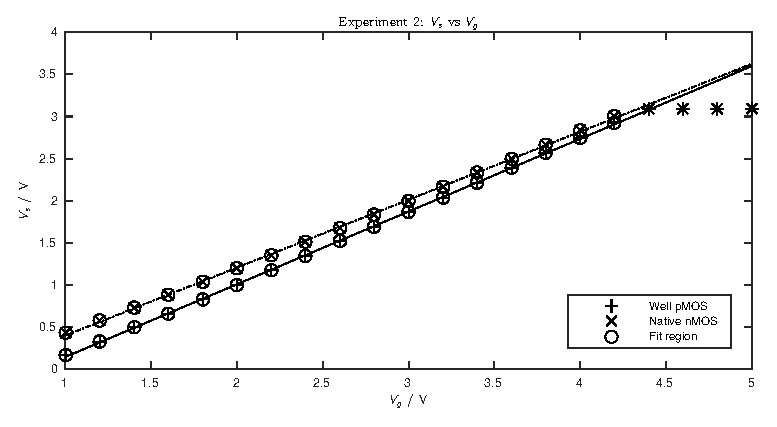
\includegraphics{ex2vsvg.eps}
    \caption{Voltage at the source terminal as a function of \(V_g\) when a current of 1 nA is forced through the transistor.
    The compliance level of 3 V is hit at 4.4 V for both transistors.}
    \label{fig:ex2vsvg}
\end{figure}
\begin{figure}
    \center
    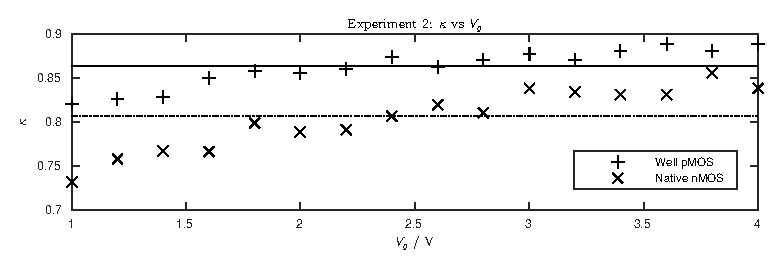
\includegraphics{ex2kappavg.eps}
    \caption{\(\kappa\) as a function of \(V_g\) when a constant current of 1 nA is forced through the transistor. \(\kappa\) 
    is obtained as the approximate derivative of the fit regions in Fig.~\ref{fig:ex2vsvg}.}
    \label{fig:ex2kappavg}
\end{figure}
\reffig{fig:ex2kappavg} shows the approximate derivative of the linear section in \reffig{fig:ex2vsvg}. This is the momentary value of
\(\kappa\). The value of \(\kappa\) is not constant because the thickness of the depletion layer changes depending on 
the gate voltage. Since \(\kappa = \frac{C_{ox}}{C_{ox}+C_{dep}}\), the value of \(\kappa\) will increase with the thickness of
the depletion layer as \(C_{dep} = \epsilon\frac{A_{dep}}{d_{dep}}\) where \(d_{dep}\) is the thickness of the layer.
The variation is relatively small and the extrapolated value from the earlier fit, also shown in \reffig{fig:ex2kappavg} is a good 
approximation. The assumption that \(\kappa\) is constant in saturation mode is therefore not entirely true, but it is a decent
approximation.

The value of \(\kappa\) obtained for both MOSFETs differ between the two experiments, however the value obtained in experiment 2
is the most accurate because it is derived without the need to assume that \(U_T=26\) mV. This assumption is unlikely to
hold as the junction temperature is most likely not room temperature.
\end{document}
